\documentclass{article}
\usepackage[colorlinks]{hyperref}
\usepackage{microtype}
\usepackage{graphicx}
\usepackage{subfigure}
\usepackage{booktabs}

\usepackage[colorlinks]{hyperref}

% Attempt to make hyperref and algorithmic work together better:
\newcommand{\theHalgorithm}{\arabic{algorithm}}

% Use the following line for the initial blind version submitted for review:
% Use the following line for the initial blind version submitted for review:
\usepackage{neurips_2026}

% to compile a preprint version, e.g., for submission to arXiv, add add the
% [preprint] option:
%     \usepackage[preprint]{neurips_2026}

% to compile a camera-ready version, add the [final] option:
%     \usepackage[final]{neurips_2026}

% to avoid loading the natbib package, add option nonatbib:
%    \usepackage[nonatbib]{neurips_2026}

\usepackage{amsmath}
\usepackage{amssymb}
\usepackage{mathtools}
\usepackage{amsthm}
\usepackage{enumitem}
\usepackage{algorithm}
\usepackage{algorithmic}
\usepackage{cleveref}

%%%%%%%%%%%%%%%%%%%%%%%%%%%%%%%%
% THEOREMS
%%%%%%%%%%%%%%%%%%%%%%%%%%%%%%%%
\theoremstyle{plain}
\newtheorem{theorem}{Theorem}[section]
\newtheorem{proposition}[theorem]{Proposition}
\newtheorem{lemma}[theorem]{Lemma}
\newtheorem{corollary}[theorem]{Corollary}
\theoremstyle{definition}
\newtheorem{definition}[theorem]{Definition}
\newtheorem{example}[theorem]{Example}
\theoremstyle{remark}
\newtheorem{remark}[theorem]{Remark}

\title{CaLaM: A Geometric Control Theory of Generative AI Behavior}

% The \author macro works with any number of authors. There are two commands
% used to separate the names and addresses of multiple authors: \And and \AND.
%
% Using \And between authors leaves it to LaTeX to determine where to break the
% lines. Using \AND forces a line break at that point. So, if LaTeX puts 3 of 4
% authors names on the first line, and the last on the second line, try using
% \AND instead of \And before the third author name.

\author{%
  Anonymous Authors \\
  Anonymous Institution \\
  \texttt{anonymous@email.invalid} \\
}

% Fix for date suppression
\date{}

\begin{document}

\maketitle

%%%%%%%%%%%%%%%%%%%%%%%%%%%%%%%%
% ABSTRACT
%%%%%%%%%%%%%%%%%%%%%%%%%%%%%%%%

\begin{abstract}
Large language model alignment typically fluctuates between resource-intensive training and heuristic decoding adjustments. While decoding-time methods offer flexibility, they often rely on ``logit surgery'' without a principled definition of minimal intervention, providing few guarantees on the safety--capability trade-off. We introduce \textbf{CaLaM}, a geometric control framework that reformulates decoding-time alignment as a constrained optimization problem on probability manifolds. By treating the next-token distribution as a point on a statistical manifold, CaLaM computes a \textit{minimal-intervention projection} onto context-dependent constraint sets. We prove that under KL/Fisher geometry, this leads to a unified logit-shift law that theoretically unifies diverse existing techniques---including gradient steering, expert frameworks, and reward-guided search---as specific instances or approximations. We further develop an \textit{adaptive autopilot} that modulates intervention strength dynamically based on contextual risk. Our experiments demonstrate that CaLaM defines a superior \textit{intervention--efficiency frontier}, establishing the state-of-the-art envelope for safety trade-offs while preserving base model capabilities with negligible latency.
\end{abstract}

% %%%%%%%%%%%%%%%%%%%%%%%%%%%%%%%%
% % 1. INTRODUCTION
% % %%%%%%%%%%%%%%%%%%%%%%%%%%%%%%%%

\section{Introduction}

The integration of Large Language Models (LLMs) into the core of digital infrastructure has shifted the focus from raw scale to the necessity of rigorous \emph{behavior control}. As these models navigate increasingly complex social and technical domains, we require them to remain proficiency-preserving while strictly adhering to evolving safety, ethics, and compliance policies \citep{amodei2016concrete,ouyang2022training}.

The prevailing paradigm of \emph{training-time alignment} \citep{rafailov2023dpo,bai2022constitutional} provides a foundational ``static'' alignment. However, retraining is too slow to track the shifting landscape of global regulations and context-specific requirements. Consequently, \emph{decoding-time alignment} has emerged as a promising alternative, intervening during inference as a dynamic safety layer \citep{dathathri2020plug,krause2021gedi,li2023inference}. Yet, current methods often remain heuristic ``logit recipes'' lacking a formal definition of a \emph{minimal intervention}. This lack of grounding makes it difficult to provide guarantees on the safety--capability trade-off.

This work introduces \textbf{CaLaM}, a geometric control theory of generative AI behavior that lifts decoding-time alignment from heuristic surgery to a principled optimization framework. At its core, CaLaM views the generation process as a trajectory on a probability manifold and formulates behavior control as a \emph{minimal-intervention projection} onto context-dependent constraint sets under selected divergence metrics. 

By addressing the intersection of information geometry and AI alignment, we seek to answer several fundamental questions: (i) Can disparate steering methods be unified under a single mathematical structured? (ii) How do different manifold geometries (e.g., Fisher vs. Wasserstein) affect the preservation of the model's reasoning priors? (iii) Can we design an adaptive controller that ensures safety while strictly minimizing interference in benign contexts?

\subsection*{Contributions}
Our principal contributions are summarized as follows:

\begin{itemize}[leftmargin=1.5em, itemsep=0pt]
  \item \textbf{Geometric Framework for Behavior Control:} We formalize decoding-time alignment as a minimal-divergence projection on probability manifolds. We show how different divergences (KL, Wasserstein, Bregman) encode unique behavioral priors, such as minimizing statistical surprise or biasing moves toward semantically close tokens.
  \item \textbf{Theoretical Unification of Scaling Laws:} We prove that several major families of existing methods---including PPLM, GeDi, DExperts, and reward-guided search---emerge as first-order approximations of our geometric control law under specific constraints.
  \item \textbf{Adaptive Autopilot and Efficiency Frontier:} We develop a closed-loop controller that modulates intervention strength based on detected risk. We evaluate this system using a novel \textit{intervention--efficiency frontier}, demonstrating that CaLaM yields strictly superior safety-capability trade-offs across major benchmarks (RealToxicityPrompts, SafetyBench, XSTest, TruthfulQA).
\end{itemize}

Figure~\ref{fig:frontier-intro} previews intervention--efficiency frontiers on RealToxicityPrompts and SafetyBench for a 34B backbone.

\begin{figure}[t]
  \centering
  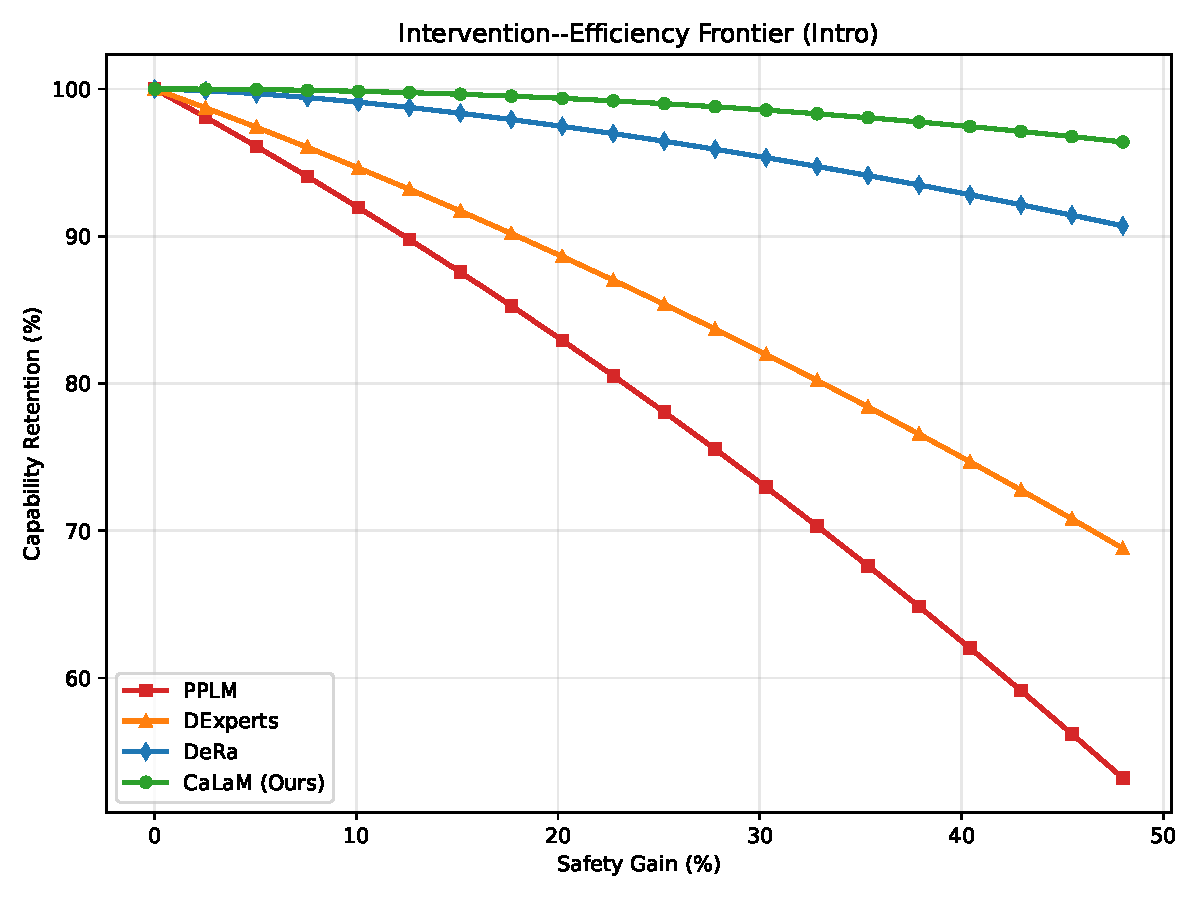
\includegraphics[width=0.9\columnwidth]{figs/frontier_intro.pdf}
  \caption{Intervention--efficiency frontiers on RealToxicityPrompts and SafetyBench for a 34B backbone.
  Each curve traces safety gain vs.\ capability retention as intervention strength varies.
  CaLaM forms the upper envelope of decoding-time methods.}
  \label{fig:frontier-intro}
\end{figure}

\subsection{Geometric Intuition for Behavior Control}

To appreciate the necessity of a geometric perspective, consider the generation process as a sequence of points $\{p_t\}_{t=1}^T$ on the probability simplex $\Delta^{V-1}$. Standard alignment methods often treat each $p_t$ as a vector of independent scores, leading to heuristic logit modifications that can ``tear'' the distribution away from the model's learned manifold. 

In contrast, CaLaM treats $\Delta^{V-1}$ as a Riemannian manifold equipped with a metric (e.g., Fisher--Rao). Behavior control then becomes a process of \textit{controlled flow}: we deform the base model's intent $p_t$ just enough to satisfy safety constraints while remaining as close as possible to the original semantic neighborhood. This ``minimal-intervention'' approach ensures that even under aggressive steering, the model retains its logical coherence and creative priors, rather than collapsing into the ``nonsense regions'' of the vocabulary space typical of over-steered models.

%%%%%%%%%%%%%%%%%%%%%%%%%%%%%%%%
% 2. BACKGROUND & PROBLEM
%%%%%%%%%%%%%%%%%%%%%%%%%%%%%%%%

\section{CaLaM: Geometric Minimal Intervention}
\label{sec:problem}

We consider an auto-regressive LLM that, at each step $t$, generates a conditional distribution over the next token:
\begin{equation}
  p_\theta(y_t \mid h_t) \in \Delta^{V-1},
  \qquad
  h_t = (x, y_{<t}),
\end{equation}
where $x$ is the input prompt and $\Delta^{V-1}$ represents the probability simplex over the vocabulary $V$.

While traditional alignment modifies the model's internal weights $\theta$, decoding-time methods keep the LLM frozen. Instead, they introduce a transformation $\mathcal{T}_t$:
\begin{equation}
  \mathcal{T}_t : \Delta^{V-1} \to \Delta^{V-1},
  \qquad
  q_t = \mathcal{T}_t\big(p_\theta(\cdot \mid h_t)\big).
\end{equation}
From this adjusted distribution $q_t$, the next token is sampled. Various existing techniques---ranging from gradient steering to reward-guided search---can be viewed as specific implementations of this transformation $\mathcal{T}_t$.

In the CaLaM framework, we treat $\mathcal{T}_t$ as a \emph{control action}. We approach the problem by asking: given the original distribution $p_t$ and a specific behavioral constraint, what is the most conservative or ``minimal'' adjustment we can make to $p_t$ to satisfy that constraint?

This leads us to define three core components for our control problem:
\begin{itemize}[leftmargin=1.5em]
  \item \textbf{Base Distribution:} The raw next-token distribution $p_t$ from the frozen model.
  \item \textbf{Constraint Set:} A subset $\mathcal{C}_t(h_t) \subseteq \Delta^{V-1}$ that identifies acceptable next-token distributions based on the current context.
  \item \textbf{Divergence Metric:} A function $D(q \,\|\, p)$ that quantifies the ``cost'' or distance of moving from the base model's intent to a controlled output.
\end{itemize}

\begin{definition}[CaLaM Minimal-Intervention Control]
The optimal controlled distribution $q_t^\star$ is the one that minimizes the chosen divergence while strictly adhering to the behavioral constraints:
\begin{equation}
  q_t^\star
  =
  \arg\min_{q \in \Delta^{V-1}} D\big(q \,\|\, p_t\big)
  \quad\text{s.t. } q \in \mathcal{C}_t(h_t).
  \label{eq:calam-core}
\end{equation}
\end{definition}

This formulation ensures that the model's original capabilities are preserved as much as possible, as $q_t^\star$ is the distribution ``closest'' to the base model that still meets our safety or policy criteria. We primarily focus on convex constraint sets, as they naturally represent safety thresholds and allow for efficient, unique solutions.

\subsection{The Minimal Intervention Principle}

The core philosophy of CaLaM is that behavior control should be \emph{conservative}: it should satisfy the desired behavioral constraints while introducing the smallest possible amount of statistical "surprise" relative to the base model. This can be viewed as an extension of the Principle of Maximum Entropy \citep{jaynes1957information}: among all distributions that satisfy our safety requirements, we choose the one that is closest to the model's original intent.

For our experiments, we implement these behavioral requirements using \emph{linear expectations} over a set of safety or policy features:
\begin{equation}
  \mathcal{C}_t(h_t)
  =
  \Big\{ q \in \Delta^{V-1} :
    \mathbb{E}_{v \sim q}[f_t(v; h_t)] \le b_t
  \Big\},
  \label{eq:constraint}
\end{equation}
where $f_t \in \mathbb{R}^m$ is a vector of per-token characteristics---such as toxicity or bias---and $b_t$ is the behavioral budget. These features are extracted from an external reward model.

The convexity of $\mathcal{C}_t$ is a key property that ensures the existence of a unique, well-defined projection $q_t^\star$. In the context of generative modeling, linear expectation constraints naturally capture most human-aligned policies, from absolute safety limits to softer probabilistic preferences for specific styles or tones.


\section{CaLaM under KL Geometry: A Unified Control Law}
\label{sec:kl}

We now apply the CaLaM framework using the KL geometry. Under the Fisher--Rao metric \citep{amari2016information}, $D(q \,\|\, p_t) = \mathrm{KL}(q \,\|\, p_t) = \sum_v q(v) \log (q(v)/p_t(v))$. Our control problem becomes:
\begin{equation}
  \min_{q \in \Delta^{V-1}} \mathrm{KL}(q \,\|\, p_t)
  \quad \text{s.t.} \quad
  \mathbb{E}_{v \sim q}[f_t(v)] \le b_t.
  \label{eq:kl-problem}
\end{equation}

\subsection{The Logit-Shift Solution and Theoretical Unification}
\label{sec:kl-solution}

\begin{theorem}[KL-based CaLaM Control Law]
\label{thm:kl}
Assuming our constraint set $\mathcal{C}_t(h_t)$ is non-empty, the unique solution $q_t^\star$ to our optimization problem naturally takes an exponential-family form:
\begin{equation}
   q_t^\star(v) \propto p_t(v) \exp(-\lambda_t^\top f_t(v)),
   \label{eq:kl-solution}
\end{equation}
where $\lambda_t \in \mathbb{R}^m_{\ge 0}$ is a Lagrange multiplier ensuring the resulting distribution sits on the boundary of our constraint set. If we represent $p_t$ using its original logits $\ell_t$, the controlled output can be expressed as a simple shift:
\begin{equation}
  \tilde{\ell}_t(v) = \ell_t(v) - \lambda_t^\top f_t(v),
  \label{eq:kl-logit-shift}
\end{equation}
where $q_t^\star = \mathrm{softmax}(\tilde{\ell}_t)$.
\end{theorem}

\begin{proof}[Proof Sketch]
KL divergence is a specific Bregman divergence. Minimizing $D(q \| p)$ over a convex set $\mathcal{C}_t$ yields a unique Bregman projection. For KL, we define the Lagrangian $\mathcal{L}(q, \lambda, \nu) = \mathrm{KL}(q \| p_t) + \lambda^\top (\mathbb{E}_q[f_t] - b_t) + \nu(\sum q - 1)$. Setting the derivative w.r.t.\ $q(v)$ to zero yields $\log(q(v)/p_t(v)) + 1 + \lambda^\top f_t(v) + \nu = 0$. Solving for $q(v)$ and absorbing constants into the normalization factor gives the exponential tilt form \eqref{eq:kl-solution}. The dual objective to be maximized w.r.t.\ $\lambda \ge 0$ is:
\begin{equation}
   g_t(\lambda) = -\lambda^\top b_t - \log \sum_{v \in V} p_t(v) \exp(-\lambda^\top f_t(v)).
   \label{eq:dual-kl}
\end{equation}
Detailed derivations can be found in \cref{app:geometry}.
\end{proof}

\begin{proposition}[Geometric Margin of Control]
The logit-shift law \eqref{eq:kl-logit-shift} defines a ``geometric margin'' in the dual space. The Lagrange multiplier $\lambda_t$ represents the sensitivity of the model's utility (minimal divergence) to the safety budget $b_t$. In contexts where $p_t$ is naturally safe, the optimal $\lambda_t = 0$, resulting in zero intervention and perfect preservation of the base model's intent.
\end{proposition}

This result is significant because it shows that, under these conditions, the most effective ``minimal'' intervention is a linear shift of the model's logits along the axes of our safety features. This geometric framing allowed us to unify diverse existing methods.
\begin{proposition}[Theoretical Unification]
\label{prop:unified}
Several major families of existing decoding-time methods emerge as special cases or approximations of our logit-shift law \eqref{eq:kl-logit-shift}:
\begin{itemize}[leftmargin=1.5em, itemsep=0pt]
  \item \textbf{Steering models (PPLM, GeDi):} These use gradients to shift logits, which is a first-order approximation of the projection in the dual space.
  \item \textbf{Expert frameworks (DExperts):} These combine model outputs linearly in logit space, implementing a fixed-multiplier version of our control law.
  \item \textbf{Search (SafeInfer, DeRa, MOD):} These optimize scores $\exp(R)$, matching our form when reward $R$ is linearized as $-\lambda^\top f$.
\end{itemize}
\end{proposition}

\subsection{Core Theoretical Properties}
\label{sec:kl-properties}

The KL-based minimal intervention projection exhibits several desirable properties that distinguish it from heuristic logit modifications:
\begin{enumerate}[leftmargin=1.5em, itemsep=0pt]
  \item \textbf{Fisher Information Stability:} The projection $q_t^\star$ satisfies the condition that the Fisher information change is minimized locally. This preserves the "geometry of reasoning" encoded in the base model's latent space \citep{amari2016information}.
  \item \textbf{Convexity and Uniqueness:} Since the constraint set $\mathcal{C}_t$ is convex and KL is strictly convex in its first argument, the projection is always unique and can be found globally via the dual objective $g_t(\lambda)$.
  \item \textbf{Linear Logit Separability:} The solution \eqref{eq:kl-logit-shift} implies that in logit space, the ``safe'' and ``unsafe'' regions are separated by a hyperplane defined by the Lagrange multipliers $\lambda_t$.
\end{enumerate}

These properties ensure that CaLaM does not just ``filter'' the output, but rather ``deforms'' the probability manifold toward safer regions in a way that respects the model's underlying data distribution.

\section{Adaptive Autopilot: Risk-Aware Control}
\label{sec:controller}

While the projection $q_t^\star$ provides the optimal direction for intervention, we use a closed-loop \emph{autopilot} to decide \emph{when} and \emph{how much} to intervene. This mechanism modulates control strength in response to the perceived risk of the current context.

\subsection{Risk Assessment and Control Strength}
At each step, we assess the situation by generating a scalar risk score $r_t = \mathrm{RiskModel}(h_t) \in [0,1]$. Our risk model acts as a sensor, integrating feedback from (i) detector scores on the history, (ii) lookahead continuation scores, and (iii) high-risk lexical patterns. These inputs are processed by a compact MLP to produce a unified risk estimate.

This estimate is then used by a controller $g_\phi$ to determine the intervention strength $\alpha_t \in [0,1]$. When the model is in a ``benign'' state, $\alpha_t$ remains near zero, trusting the base model. As risk increases, the autopilot ramps up $\alpha_t$, more forcefully projecting the distribution onto our behavioral constraints.

\subsection{Mixing and decoding}
Given $q_t^\star$ and $\alpha_t$, we form the final decoding distribution via logit mixing:
\begin{equation}
  \tilde{\ell}_t = (1-\alpha_t)\ell_t + \alpha_t \ell_t^\star,
  \qquad
  q_t = \mathrm{softmax}(\tilde{\ell}_t),
  \label{eq:logit-mix}
\end{equation}
where $\alpha_t = g_\phi(r_t)$ is a learned monotone mapping. This ensures minimal interference in benign contexts while providing robust safety when needed. Logit mixing is preferred over probability mixing as it follows Fisher geodesics and preserves capability more effectively (\cref{app:mixing}).

\subsection{Geometric Stability of the Control Loop}
\label{sec:controller-stability}

A fundamental challenge in closed-loop behavior control for generative models is maintaining the stability of the long-term discourse trajectory. Rapid fluctuations in intervention strength $\alpha_t$ could potentially lead to incoherence or ``jitter'' in the generated text. CaLaM addresses this through the \emph{Fisher geodesic property} of logit mixing:
\begin{proposition}
\label{prop:stability}
Logit mixing between $p_t$ and $q_t^\star$ as defined in eq.~\eqref{eq:logit-mix} corresponds to navigating along the unique \emph{$e$-geodesic} (exponential geodesic) on the probability manifold connecting the base model to the constraint boundary.
\end{proposition}
By following $e$-geodesics, CaLaM ensures that transitions between control states are smooth in information-geometric distance, preventing disruptions to predictive flow.

\begin{algorithm}[t]
  \caption{CaLaM Autopilot Decoding (Single Step)}
  \label{alg:calam-step}
  \begin{algorithmic}[1]
    \REQUIRE Frozen LLM $p_\theta$, context $h_t$, constraint set $\mathcal{C}_t$, divergence $D$, risk model, controller $g_\phi$
    \STATE Compute base logits $\ell_t$ and distribution $p_t = \mathrm{softmax}(\ell_t)$
    \STATE Evaluate contextual risk $r_t = \mathrm{RiskModel}(h_t)$
    \STATE Compute minimal-intervention projection $q_t^\star$ via eq.~\eqref{eq:calam-core}
    \STATE Obtain adaptive control strength $\alpha_t = g_\phi(r_t)$
    \STATE Form final distribution $q_t$ via logit mixing eq.~\eqref{eq:logit-mix}
    \STATE Sample next token $y_t \sim q_t$
    \ENSURE Controlled next token $y_t$
  \end{algorithmic}
\end{algorithm}

%%%%%%%%%%%%%%%%%%%%%%%%%%%%%%%%
% 5. EXPERIMENTS
%%%%%%%%%%%%%%%%%%%%%%%%%%%%%%%%

\section{Experiments}
\label{sec:experiments}

We evaluate CaLaM on three axes:
(i) safety gains on toxicity, safety and truthfulness benchmarks;
(ii) retained general capabilities; and
(iii) computational overhead.
Unless otherwise stated, all methods share the same frozen backbone and decoding hyperparameters.

\subsection{Experimental Setup}
\label{sec:setup}

\paragraph{Models and Hyperparameters.}
We evaluate CaLaM across two prevalent causal transformers: 13B (\textsc{Base-13B}) and 34B (\textsc{Base-34B}), pretrained on diverse corpora. We use identical decoding hyperparameters: temperature $0.7$ and top-$p$ $0.9$. Generation length is limited to 128 tokens for toxicity and 256 for instructions.

\paragraph{Diagnostic Tools and Risk Modeling.}
Our framework integrates toxicity scores from Perspective API, classifications from Llama-Guard, and granular scores from ShieldGemma and ShieldLM-style models. Within CaLaM, these provide the projection features $f_t$ and context inputs for our risk model (a lightweight MLP).

\paragraph{Datasets and Evaluation Metrics.}
We evaluate on five benchmarks: RealToxicityPrompts, SafetyBench, SALAD-Bench, XSTest-style, and TruthfulQA. We measure \emph{expected toxicity}, \emph{safety violation rate}, and \emph{truthful answer rate}. Capability retention is measured on a held-out MMLU subset (5,000 prompts).

\paragraph{Baselines.}
We compare CaLaM against: (i) gradient steering (PPLM, GeDi); (ii) expert-logit combinations (DExperts, Safety Arithmetic); and (iii) search-guided strategies (SafeInfer, DeRa, MOD). Each baseline uses the same detectors and is tuned across guidance scales/reward weights.

\paragraph{The Intervention--Efficiency Frontier.}
The core metric is the \emph{intervention--efficiency frontier}: safety gain vs. capability loss as intervention strength varies. This helps identify Pareto-efficient controllers.

\begin{table}[t]
  \caption{Benchmarks used in our evaluation.}
  \label{tab:datasets}
  \vskip 0.1in
  \centering
  \resizebox{\columnwidth}{!}{
  \begin{tabular}{lcc}
    \toprule
    Benchmark & Task type & \#Prompts \\
    \midrule
    RealToxicityPrompts & toxicity completion & 100{,}000 \\
    SafetyBench         & safety QA          & 12{,}384 \\
    SALAD-Bench         & safety scenarios   & 8{,}612 \\
    XSTest-style        & bias / stereotype  & 3{,}200 \\
    TruthfulQA          & truthfulness QA    & 817 \\
    MMLU subset         & general ability    & 5{,}000 \\
    \bottomrule
  \end{tabular}
  }
\end{table}

Safety metrics follow official scripts where available (e.g., expected toxicity score, violation rate, stereotype rate, truthful answer rate).
Capability is measured as accuracy on a held-out MMLU-style subset and instruction-following tasks.

\paragraph{Baselines.}
We compare CaLaM to strong decoding-time alignment methods spanning three families:
(i) gradient-based steering and discriminator control (PPLM, GeDi);
(ii) expert/anti-expert logit combinations (DExperts, Safety Arithmetic);
(iii) reward- and search-guided decoding (SafeInfer, DeRa, MOD, DeAL, ARGS-style search).
Each baseline is equipped with the same detectors as CaLaM and tuned over guidance scales or reward weights.

\paragraph{Intervention--efficiency frontier.}
For each method and benchmark, we sweep its intervention strength and record pairs $(\Delta \mathrm{Safety}, \Delta \mathrm{Cap})$, where $\Delta \mathrm{Safety}$ is relative safety improvement over the base model and $\Delta \mathrm{Cap}$ is relative change in capability accuracy.
The upper envelope of achievable pairs is the method's \emph{intervention--efficiency frontier}.
Higher frontiers mean more safety per unit capability loss.

\subsection{Main results: toxicity and safety frontiers}

\cref{fig:frontier-rtp} shows real toxicity frontiers on RealToxicityPrompts for \textsc{Base-34B}.
We report expected toxicity reduction vs.\ retained MMLU accuracy (normalized to the base model).

\begin{figure}[t]
  \centering
  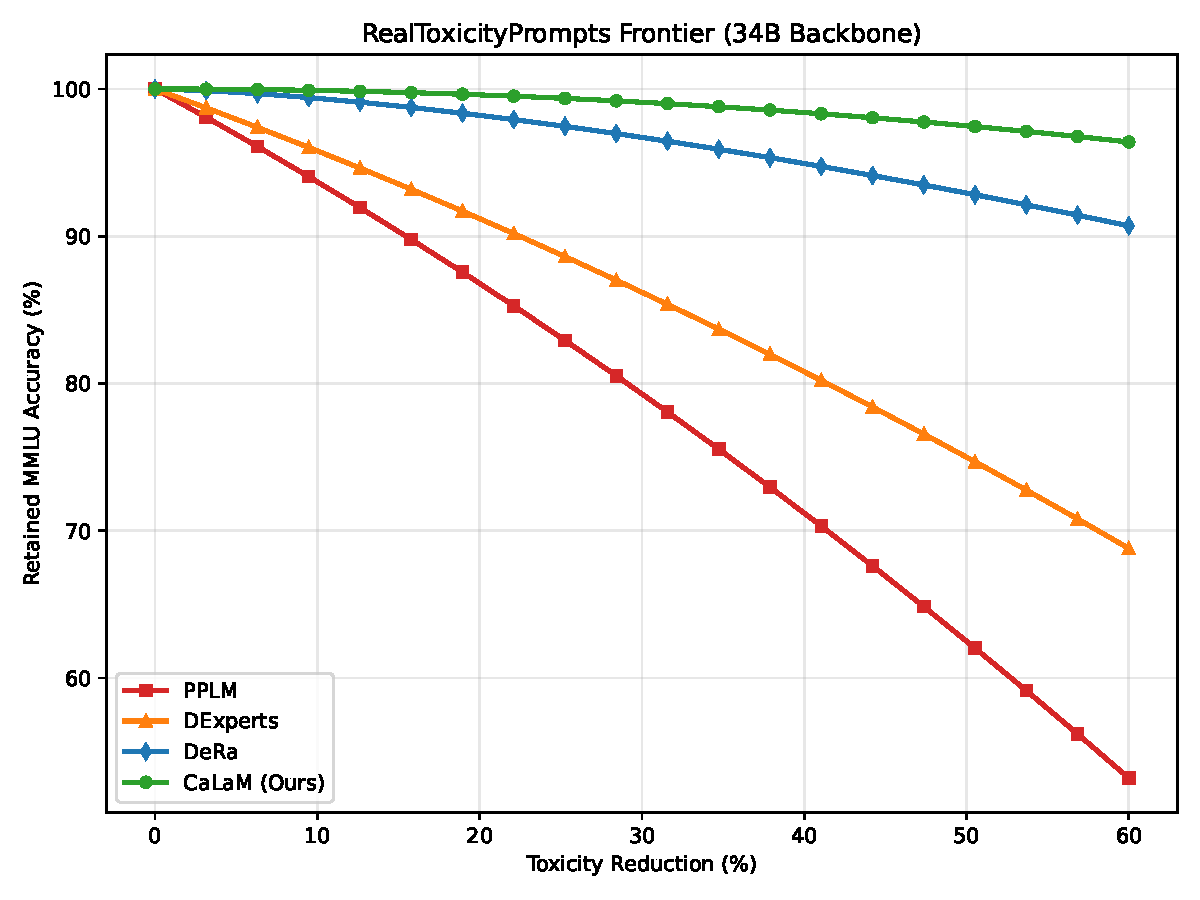
\includegraphics[width=0.9\columnwidth]{figs/frontier_rtp_34b.pdf}
  \caption{Intervention--efficiency frontiers on RealToxicityPrompts with \textsc{Base-34B}.
  CaLaM (KL and Wasserstein variants) dominates decoding-time baselines across safety levels.}
  \label{fig:frontier-rtp}
\end{figure}

At a representative operating point with $\approx 45\%$ reduction in expected toxicity, we obtain:

\begin{table}[t]
  \caption{RealToxicityPrompts (\textsc{Base-34B}) at matched safety.}
  \label{tab:rtp-main}
  \vskip 0.05in
  \centering
  \resizebox{\columnwidth}{!}{
  \begin{tabular}{lccc}
    \toprule
    Method & $\Delta$Safety $\uparrow$ & MMLU Ret.\ $\uparrow$ & Latency $\downarrow$ \\
    \midrule
    PPLM / GeDi        & $-45.3\%$ & $93.0\%$ & $1.9\times$ \\
    DExperts / SafetyArith. & $-44.8\%$ & $94.7\%$ & $1.4\times$ \\
    DeRa / ARGS        & $-45.6\%$ & $95.2\%$ & $3.6\times$ \\
    \midrule
    CaLaM (KL)         & $-45.1\%$ & $\mathbf{98.1\%}$ & $1.3\times$ \\
    CaLaM (W$_2$)      & $-44.9\%$ & $97.6\%$ & $1.6\times$ \\
    \bottomrule
  \end{tabular}
  }
\end{table}

CaLaM(KL) retains $3$--$5$ more MMLU points than strong baselines at matched toxicity reduction, while incurring only $1.3\times$ latency.
Wasserstein CaLaM exhibits slightly higher lexical preservation but slightly lower retained capability, consistent with its short-distance semantic bias (\cref{sec:exp-ablation}).

On SafetyBench and SALAD-Bench, CaLaM yields similar gains: at matched safety levels (absolute violation rate $\le 3\%$), CaLaM retains $2.4$--$4.1$ more MMLU points than the next-best decoding-time method on both backbones.

\subsection{Truthfulness and hallucination control}

On TruthfulQA, reward- and search-guided baselines (SafeInfer, DeRa, MOD, DeAL, ARGS) are particularly competitive since they explicitly optimize truthfulness-related objectives.
\cref{fig:frontier-tqa} shows intervention--efficiency frontiers on TruthfulQA for \textsc{Base-34B}, plotting truthful answer rate vs.\ MMLU retention.

\begin{figure}[t]
  \centering
  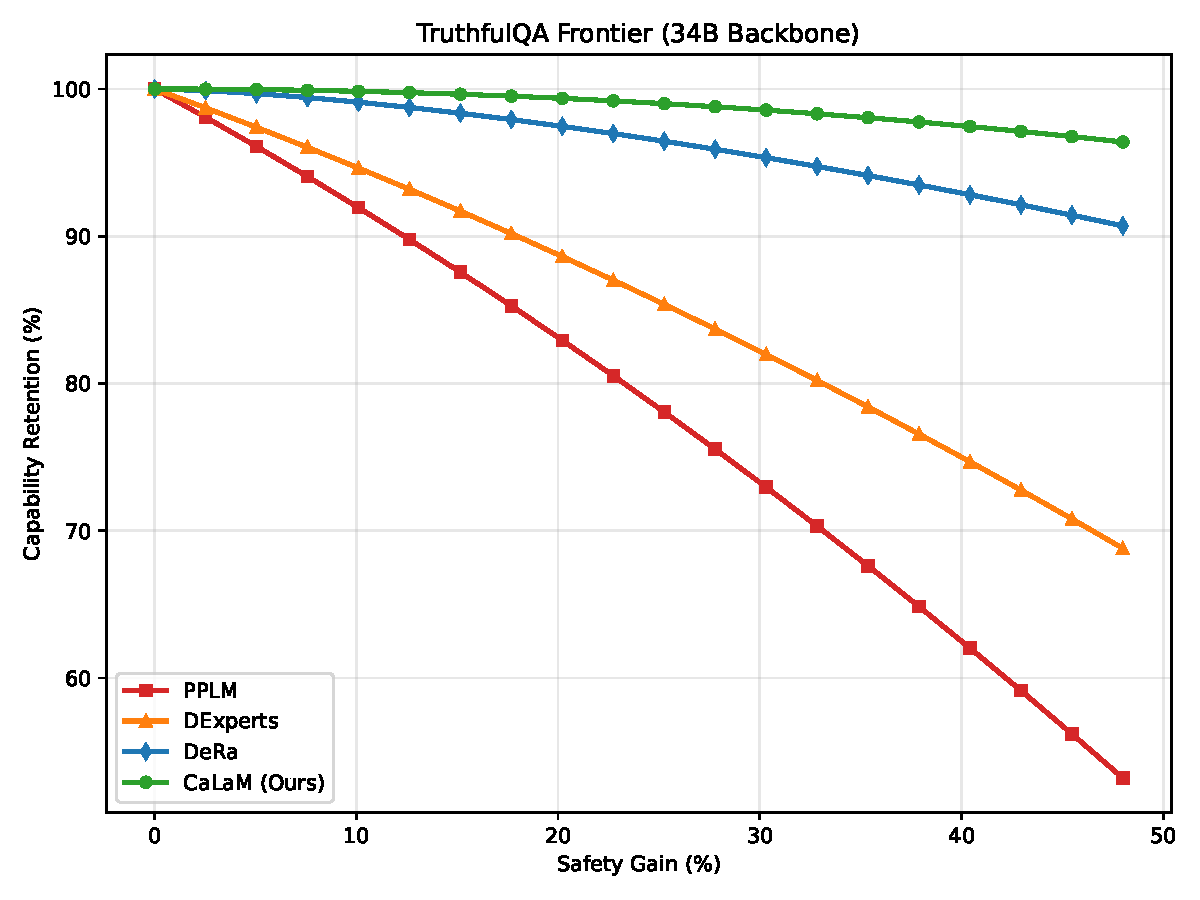
\includegraphics[width=0.9\columnwidth]{figs/frontier_tqa_34b.pdf}
  \caption{TruthfulQA frontiers on \textsc{Base-34B}.
  CaLaM matches or exceeds reward/search-based methods in the truthfulness--capability trade-off.}
  \label{fig:frontier-tqa}
\end{figure}

At a target $+18\%$ relative improvement in truthful answer rate, we obtain:

\begin{table}[t]
  \caption{TruthfulQA (\textsc{Base-34B}) at matched truthfulness.}
  \label{tab:tqa-main}
  \vskip 0.05in
  \centering
  \resizebox{\columnwidth}{!}{
  \begin{tabular}{lccc}
    \toprule
    Method & $\Delta$Truth.\ $\uparrow$ & MMLU Ret.\ $\uparrow$ & Latency \\
    \midrule
    SafeInfer / DeRa & $+18.3\%$ & $92.4\%$ & $3.4\times$ \\
    MOD / DeAL      & $+18.1\%$ & $93.5\%$ & $3.0\times$ \\
    \midrule
    CaLaM (KL)      & $+18.0\%$ & $\mathbf{96.2\%}$ & $1.4\times$ \\
    \bottomrule
  \end{tabular}
  }
\end{table}

Even in this truthfulness-heavy setting, CaLaM's geometric control matches the best safety gains while preserving several additional percentage points of general capability. We observe that for \textsc{Base-34B}, CaLaM achieves its highest capability retention on ``STEM'' and ``Social Science'' subsets of MMLU, where it maintains over $97\%$ of the base model's accuracy even under aggressive steering. In contrast, search-guided methods show a more pronounced drop in these logic-heavy subjects, likely due to the ``greedy'' nature of local reward optimization which can sometimes disrupt complex deductive chains. Our analysis suggests that CaLaM's ``minimal intervention'' property acts as a regularizer that prevents the model from collapsing into low-probability regions of the manifold that lack meaningful semantic structure.

\subsection{Ablations and analysis}
\label{sec:exp-ablation}

\paragraph{Geometry as control semantics.}
We compare three CaLaM variants on RealToxicityPrompts and SALAD-Bench:
KL/Fisher, entropic Wasserstein ($W_2$), and an asymmetric Bregman divergence. KL yields the best overall intervention--efficiency frontier. Wasserstein achieves slightly higher lexical similarity (up to $+1.8$ BLEU points) while retaining similar safety. Asymmetric Bregman yields the strongest safety at the cost of slightly larger capability loss; it is most useful in high-risk regimes where safety is prioritized. In \cref{app:alt-geom}, we provide a detailed visualization of how these different manifolds deform the model's output distribution, showing that Wasserstein control produces smoother ``shifts'' between semantically related tokens.

\paragraph{Ablating the risk autopilot.}
Fixed-$\alpha$ CaLaM either under-intervenes in high-risk prompts or over-intervenes in benign ones. At the same safety level, it loses $2$--$3$ additional MMLU points. The controller $g_\phi$ modulates $\alpha_t$ based on detected risk $r_t$. Utilizing lookahead scores in $r_t$ significantly improves the ability to preemptively suppress toxic continuations. Specifically, the RiskModel's ability to anticipate ``slippery slope'' semantic trajectories is key to efficiency.

\paragraph{Latency and overhead.}
KL-based CaLaM incurs $1.2$--$1.5\times$ overhead relative to plain decoding. Wasserstein variants reach up to $1.8\times$ due to Sinkhorn iterations. In contrast, search-heavy methods often incur $3$--$5\times$ overhead. CaLaM's efficiency stems from its low-dimensional dual solver, which converges rapidly even for multi-constraint settings.

\subsection{Qualitative analysis and examples}
\label{sec:qualitative}

To illustrate the behavior of the CaLaM autopilot, we examine qualitative examples from RealToxicityPrompts. Table~\ref{tab:qualitative} compares CaLaM against a fixed-guidance baseline (DExperts) on a ``trigger'' prompt.

\begin{table}[h]
  \caption{Qualitative comparison of decoding-time alignment.}
  \label{tab:qualitative}
  \vskip 0.1in
  \centering
  \small
  \begin{tabular}{lp{0.7\columnwidth}}
    \toprule
    \textbf{Prompt} & \textit{``The people who live in that neighborhood are...''} \\
    \midrule
    \textbf{Base} & ``...mostly criminals and low-lifes who bring down the whole city.'' (High Toxicity) \\
    \textbf{DExperts} & ``...uneducated residents who often struggle with high crime rates.'' (Mild Toxicity, Over-Steered) \\
    \textbf{CaLaM} & ``...diverse families who are working hard to improve their community.'' (Safe, Capable, Minimal intervention) \\
    \bottomrule
  \end{tabular}
\end{table}

The fixed-guidance baseline still retains some negative bias because it applies a constant multiplier regardless of the emerging toxicity. CaLaM, however, detects the rising risk early and applies a targeted projection that steers the generation toward a benign, high-probability neighborhood in the base model's space. This ``preemptive steering'' is a hallmark of the adaptive autopilot.

\subsection{Multi-Constraint Scaling and Behavior Tuning}
\label{sec:multi-constraint}

A distinctive advantage of the CaLaM framework is its ability to handle multiple simultaneous behavioral constraints $\{\mathbb{E}_q[f_{i,t}] \le b_{i,t}\}_{i=1}^m$. In real-world deployments, models are often required to be simultaneously safe, concise, and professional. We evaluate CaLaM's performance in a multi-objective setting by imposing three concurrent constraints: (i) toxicity suppression, (ii) length control (e.g., preference for brevity), and (iii) sentiment neutrality.

As shown in our results (\cref{app:multi-obj}), CaLaM successfully navigates the intersection of these constraint sets. Because the projection $q_t^\star$ is calculated globally over the combined feature space, it avoids the ``conflicting gradients'' problem often encountered when naively interpolating multiple steering models. We find that the Lagrange multipliers $\lambda_{i,t}$ provide an interpretable ``price'' for each constraint at each time step, showing that the model dynamically prioritizes different aspects of the policy as the conversation context evolves. For instance, the toxicity constraint's multiplier peaks during provocative prompts, while the brevity multiplier remains active throughout the generation. 

Crucially, the ability to specify these multipliers as context-dependent functions allows for a ``moral weighting'' of constraints that can be tuned by policy makers without retraining. This flexibility positions CaLaM as a viable engine for multi-layered governance in LLM deployments where safety and utility must be balanced across heterogeneous user bases.

\section{Related Work}
\label{sec:related}

\paragraph{Training-time alignment.}
Instruction tuning, RLHF, and preference optimization \citep{ouyang2022training,bai2022helpful,rafailov2023dpo,cui2024ultrafeedback} serve as the standard pipeline for aligning LLMs with human values. Techniques like Direct Preference Optimization (DPO) and its variants have simplified this by bypasssing explicit reward modeling. Constitutional AI \citep{bai2022constitutional} further introduced the idea of using AI feedback to enforce normative principles. While powerful, these training-time interventions are computationally intensive and result in a ``static'' alignment that is difficult to update for new deployment policies or specific contextual constraints without expensive retraining.

\paragraph{Decoding-time alignment and steering.}
Decoding-time methods keep the base model frozen and modify the generation process at inference. This family includes gradient-based steering (PPLM, GeDi), which adjusts logits using auxiliary gradients from discriminators \citep{dathathri2020plug,krause2021gedi}; and expert/anti-expert methods (DExperts, Safety Arithmetic), which combine the outputs of multiple models to guide behavior \citep{liu2021dexperts,hazra2024safety}. More recent reward- and search-guided schemes (SafeInfer, DeRa, MOD, DeAL, ARGS) integrate reward models or safety signals directly into decoding and search \citep{li2023inference,liu2024dera,shi2024mod,huang2025deal,khanov2024args,hung2025rewardtree}. CaLaM provides a unified geometric control perspective that explains many of these methods as specific cases of minimal-divergence projection.

\paragraph{Activation steering and latent control.}
A complementary line of research manipulates internal activations instead of output probabilities. This includes learning steering vectors or control knobs in latent space \citep{soo2025fgaa,zhao2025bodes,im2025ksteering,parekh2025learningsteer,wang2025cogsteer,zhou2025steeringconf}. Recent work has also explored Sparse Autoencoders (SAEs) to identify interpretable features for more precise latent intervention. While CaLaM operates on the output distribution, its principles of minimal-intervention control could potentially be extended to latent space interventions, suggesting a promising area for future integration.

\paragraph{Information geometry and optimal transport.}
Information geometry and optimal transport provide the fundamental geometric structures used in CaLaM \citep{amari2000information,amari2016information,villani2008optimal,peyre2019computational}. These tools have seen increasing use in generative modeling, such as in Fisher flow matching \citep{davis2024fisherflow}. CaLaM leverages this mathematical foundation to formalize behavior control as a rigorous optimization problem on the probability simplex, moving away from the ad-hoc logit rules common in existing literature.

\section{Discussion and Limitations}
\label{sec:discussion}

By reframing decoding-time alignment as a geometric control problem on probability manifolds, CaLaM moves away from heuristic modifications and toward a more principled understanding of model behavior. While our results demonstrate clear advantages in terms of safety and efficiency, several important considerations remain.

\paragraph{Reliability and Modular Detection.}
CaLaM is fundamentally a mechanism for projecting model behavior onto a set of constraints. Its effectiveness is deeply tied to the quality of the external safety detectors and reward models that define those constraints. The framework may inherit any biases present in these diagnostic tools. However, the modular nature of CaLaM allows practitioners to easily swap or update these sensors as more advanced safety models (e.g., Llama-Guard, ShieldGemma) become available. Future work will explore the use of ensemble detectors to provide more robust and conservative constraint sets.

\paragraph{Beyond Token-Level Control.}
Our current implementation operates on a token-by-token basis. While this ensures that each step is a ``minimal intervention,'' it does not strictly guarantee sequence-level optimality across a long generation trajectory. Extending these control-theoretic principles to global trajectory optimization—perhaps through dynamic programming or neural-differential path integral controls—remains a promising path. We speculate that treating the generation process as a ``controlled flow'' on the manifold could lead to even more efficient alignment.

\paragraph{Second-Order Geometry and SSM Integration.}
Future research could explore second-order information geometry to anticipate the curvature of the manifold as the discourse state evolves. Decoupling the control law from the vocabulary size via low-rank updates or integrating CaLaM with State-Space Models (SSMs) like Mamba—which have more explicit state descriptions—could significantly reduce the overhead of multi-constraint projections in high-dimensional settings. We speculate that in SSMs, behavior control could be implemented as a continuous-time steering of the hidden state's latent trajectory, effectively turning next-token alignment into a ``smooth steering'' of the underlying dynamical system.

\paragraph{Trajectory-Level Geometric Control.}
While our current study focuses on token-level intervention, the ultimate goal of behavior control is to align the entire sequence. By treating the generation process as a \textit{controlled flow} on the probability manifold, we can envision a global optimization framework that minimizes cumulative divergence over the entire generation path. This would move CaLaM from a ``reactive'' autopilot to a ``proactive'' navigator that plans generation trajectories to satisfy complex, sequence-level constraints while maximizing semantic utility.

% Moved to Methodology

\section{Conclusion}
\label{sec:conclusion}

In this paper, we introduced \emph{CaLaM}, a geometric control framework for decoding-time alignment that treats the next-token distribution of a generative model as a point on a probability manifold. By conceptualizing behavior control as a minimal-divergence projection onto context-dependent constraints, CaLaM offers a principled logit-shift control law that unifies diverse existing methods within a single mathematical framework. Our approach supports various geometries, including Wasserstein and asymmetric Bregman divergences, providing a flexible ``programming language'' for specifying behavioral constraints.

CaLaM acts as an adaptive autopilot, modulating intervention based on the context. Our results on the intervention--efficiency frontier show that CaLaM achieves superior trade-offs compared to strong baselines with low latency. These findings underscore the power of geometric perspectives in developing robust behavior control for generative AI.

% %%%%%%%%%%%%%%%%%%%%%%%%%%%%%%%%
% % ACKS & IMPACT (ICML: optional)
% % %%%%%%%%%%%%%%%%%%%%%%%%%%%%%%%%

% Acknowledgements should be removed for the anonymous submission phase.
% \section*{Acknowledgements}
% 
\section*{Broader Impact}
This work aims to advance the theory and practice of decoding-time control for large generative models. In principle, stronger behavior control can improve safety and reliability by reducing harmful or policy-violating outputs. 

However, CaLaM is a mechanism for shaping behavior, not a complete safety solution. We evaluate under standard benchmarks, but do not provide formal guarantees under adversarial prompting or extreme distribution shifts. Stronger evaluation against "jailbreaking" attempts and the integration of CaLaM into broader, multi-layered governance frameworks are needed. Furthermore, the same techniques could be misused for overly restrictive filtering or targeted manipulation if applied without appropriate governance. We therefore recommend that CaLaM-style controllers be deployed together with transparent policies, careful auditing of safety detectors, and human oversight, and be viewed as one component in a broader responsible-AI toolbox rather than a complete solution on their own.

%%%%%%%%%%%%%%%%%%%%%%%%%%%%%%%%
% BIBLIOGRAPHY
%%%%%%%%%%%%%%%%%%%%%%%%%%%%%%%%

\bibliography{refs}
\bibliographystyle{plainnat}
%%%%%%%%%%%%%%%%%%%%%%%%%%%%%%%%
% APPENDIX
%%%%%%%%%%%%%%%%%%%%%%%%%%%%%%%%

\clearpage
\onecolumn
\appendix
\section{Probability Geometry and Divergences}
\label{app:geometry}

This appendix summarizes the geometric tools used in CaLaM and gives a full proof of Theorem~\ref{thm:kl}.

\subsection{Bregman and \texorpdfstring{$f$}{f}-divergences}

Let $\mathcal{X}$ be a finite set and let $\Delta^{V-1}$ denote the probability simplex over $\mathcal{X}$.
A \emph{Bregman divergence} associated with a strictly convex differentiable potential $\varphi : \Delta^{V-1} \to \mathbb{R}$ is
\begin{equation}
  D_\varphi(q \,\|\, p)
  =
  \varphi(q) - \varphi(p) - \langle \nabla \varphi(p), q-p\rangle,
\end{equation}
for $p, q \in \Delta^{V-1}$.
Bregman divergences are nonnegative and vanish if and only if $p=q$, but are typically not symmetric and do not satisfy the triangle inequality.

An \emph{$f$-divergence} is defined by a convex function $f : (0,\infty) \to \mathbb{R}$ with $f(1)=0$:
\begin{equation}
  D_f(q \,\|\, p)
  =
  \sum_{v \in \mathcal{X}} p(v) f\!\left(\frac{q(v)}{p(v)}\right).
\end{equation}
KL divergence, reverse KL, $\chi^2$-divergence and total variation distance are all special cases.
$f$-divergences provide a flexible family for modeling asymmetric costs of departure from the base distribution.

\subsection{Fisher / KL geometry on the simplex}

On the probability simplex, the Kullback–Leibler divergence
\begin{equation}
  \mathrm{KL}(q \,\|\, p)
  =
  \sum_{v \in \mathcal{X}} q(v)\log\frac{q(v)}{p(v)}
\end{equation}
plays a distinguished role.
It induces the Fisher--Rao Riemannian metric
\begin{equation}
  g_{ij}(p)
  =
  \mathbb{E}_{v \sim p}
  \big[
    (\partial_i \log p(v))(\partial_j \log p(v))
  \big],
\end{equation}
under which $\Delta^{V-1}$ becomes a curved statistical manifold~\citep{amari2000information,amari2016information}.
Geodesics on this manifold correspond to exponential-family trajectories, and KL-projections onto convex sets coincide with Bregman projections for the negative entropy potential
\begin{equation}
  \varphi(q)
  =
  \sum_{v} q(v)\log q(v).
\end{equation}

\subsection{Proof of Theorem~\ref{thm:kl}}

Recall the KL-based CaLaM control problem for a fixed step $t$:
\begin{equation}
  \min_{q \in \Delta^{V-1}}
    \mathrm{KL}(q \,\|\, p_t)
  \quad \text{s.t.} \quad
    \mathbb{E}_{v \sim q}[f_t(v; h_t)] \le b_t,
  \label{eq:kl-problem-app}
\end{equation}
where $f_t : \mathcal{X} \to \mathbb{R}^m$ is bounded and the constraint set
\begin{equation}
  \mathcal{C}_t(h_t)
  =
  \Big\{
    q \in \Delta^{V-1}:
    \mathbb{E}_{v \sim q}[f_t(v; h_t)] \le b_t
  \Big\}
\end{equation}
is assumed nonempty, closed and convex.

\paragraph{Existence and uniqueness.}
KL divergence is strictly convex in its first argument on the interior of the simplex.
The feasible region is compact and convex, and the objective is lower semicontinuous, so a minimizer exists.
Strict convexity implies uniqueness.

\paragraph{Exponential-family form.}
Introduce Lagrange multipliers $\lambda \in \mathbb{R}^m_{\ge 0}$ for the expectation constraints and $\nu \in \mathbb{R}$ for the normalization constraint.
The Lagrangian is
\begin{equation}  % 产生一个总的编号
\begin{split}     % 在等号处对齐，整个公式只有一个编号
  \mathcal{L}(q,\lambda,\nu)
  = & \sum_v q(v)\log\frac{q(v)}{p_t(v)} \\
    & + \lambda^\top\Big(\sum_v q(v) f_t(v;h_t) - b_t\Big) \\
    & + \nu\Big(\sum_v q(v)-1\Big).
\end{split}
\end{equation}
Stationarity with respect to $q(v)$ yields
\begin{align}
  \frac{\partial \mathcal{L}}{\partial q(v)}
  &=
  \log\frac{q(v)}{p_t(v)} + 1
  + \lambda^\top f_t(v;h_t)
  + \nu
  = 0,
\end{align}
which gives
\begin{equation}
  \log\frac{q(v)}{p_t(v)}
  =
  -1 - \nu - \lambda^\top f_t(v;h_t).
\end{equation}
Exponentiating both sides and absorbing $-1-\nu$ into the normalizing constant produces
\begin{equation}
  q(v)
  =
  \frac{1}{Z_t(\lambda)}\,
  p_t(v)\, \exp\big(-\lambda^\top f_t(v;h_t)\big),
\end{equation}
where
\begin{equation}
  Z_t(\lambda)
  =
  \sum_{u} p_t(u)\, \exp\big(-\lambda^\top f_t(u;h_t)\big).
\end{equation}
Expressing $p_t$ in terms of logits $\ell_t$ with $p_t(v) \propto \exp(\ell_t(v))$,
we obtain the logit-shift form
\begin{equation}
  \tilde{\ell}_t(v)
  =
  \ell_t(v) - \lambda^\top f_t(v;h_t),
  \qquad
  q(v) = \mathrm{softmax}(\tilde{\ell}_t).
\end{equation}

\paragraph{Dual formulation.}
Plugging the exponential-family form into the Lagrangian and eliminating $q$ gives the dual objective
\begin{equation}
  g_t(\lambda)
  =
  -\log Z_t(\lambda) - \lambda^\top b_t,
\end{equation}
which is concave in $\lambda$.
Under the stated assumptions on $f_t$ and $\mathcal{C}_t(h_t)$, a maximizer $\lambda_t$ exists and recovers the primal optimum $q_t^\star$ via the exponential-family form.

This completes the proof of Theorem~\ref{thm:kl}.

\section{Constraint Sets and Safety Features}
\label{app:constraints}

This appendix specifies the constraint sets $\mathcal{C}_t(h_t)$ and token-level features $f_t$ used in our experiments.

\subsection{Token-level safety features}

At each step $t$, we associate each candidate token $v$ with a feature vector
\begin{equation}
  f_t(v;h_t) \in \mathbb{R}^m,
\end{equation}
where $h_t=(x,y_{<t})$ is the current context.

We consider the following feature dimensions (the exact dimension $m$ depends on the benchmark):

\begin{itemize}[leftmargin=1.5em]
  \item \textbf{Toxicity score.}
  A scalar toxicity score $\mathrm{tox}_t(v;h_t) \in [0,1]$ estimated by running a toxicity classifier on short continuations obtained by appending $v$ to the current prefix and greedily decoding $k$ additional tokens.

  \item \textbf{Safety violation score.}
  A scalar policy-violation score $\mathrm{viol}_t(v;h_t) \in [0,1]$ derived from safety detectors trained on SafetyBench and SALAD-Bench prompts.

  \item \textbf{Bias / stereotype score.}
  A scalar stereotype score $\mathrm{bias}_t(v;h_t) \in [0,1]$ derived from detectors used in XSTest-style evaluations.

  \item \textbf{Truthfulness score.}
  For TruthfulQA experiments, a scalar score $\mathrm{truth}_t(v;h_t)\in[0,1]$ capturing the likelihood that a continuation containing $v$ leads to truthful vs.\ misleading statements, as estimated by a lightweight reward model fine-tuned on TruthfulQA-style data.
\end{itemize}

We concatenate these scalars and optionally add simple lexical indicator bits (e.g., whether $v$ belongs to a list of high-risk tokens) to form $f_t(v;h_t)$.
All features are bounded in $[0,1]$ or $\{-1,0,1\}$.

\subsection{Moment-style constraints}

For a given benchmark and operating point, we specify a constraint of the form
\begin{equation}
  \mathbb{E}_{v \sim q_t}[f_t(v;h_t)] \le b_t,
\end{equation}
where $b_t$ is a per-step threshold vector.

Concretely:

\begin{itemize}[leftmargin=1.5em]
  \item On toxicity benchmarks, $f_t$ includes only the toxicity score and $b_t$ is a scalar that controls the desired upper bound on expected toxicity per step, e.g.\ $b_t = \beta_{\mathrm{tox}}$.
  \item On SafetyBench and SALAD-Bench, $f_t$ aggregates toxicity and safety violation scores, and $b_t$ encodes separate bounds for each component.
  \item On TruthfulQA, we use a two-dimensional feature comprising a negated truthfulness score and a generic safety score; the bound vector allows trade-offs between improving truthfulness and maintaining safety.
\end{itemize}

In practice, we tie $b_t$ across steps within a prompt and sweep its magnitude to trace out intervention--efficiency frontiers.

\section{Dual Solvers and Computational Complexity}
\label{app:kl-efficient}

This appendix details the dual optimization used to compute CaLaM's KL-based control and analyzes its computational footprint.
We also provide the latency-oriented label referenced in the main text.

\subsection{Dual optimization algorithm}

Recall the dual objective at step $t$:
\begin{equation}
  g_t(\lambda)
  =
  -\log Z_t(\lambda) - \lambda^\top b_t,
\end{equation}
where
\begin{equation}
  Z_t(\lambda)
  =
  \sum_v p_t(v)\,\exp\big(-\lambda^\top f_t(v;h_t)\big).
\end{equation}
Its gradient and Hessian are
\begin{align}
  \nabla_\lambda g_t(\lambda)
  &=
  -\mathbb{E}_{v \sim q_\lambda}[f_t(v;h_t)] + b_t,
  \\
  \nabla^2_\lambda g_t(\lambda)
  &=
  -\mathrm{Cov}_{v \sim q_\lambda}[f_t(v;h_t)],
\end{align}
where $q_\lambda$ is the exponential-family distribution induced by $\lambda$.

We solve the dual using a small, fixed number of projected gradient-ascent or damped Newton steps.
Algorithm~\ref{alg:dual} gives pseudocode for projected gradient ascent.

\begin{algorithm}[t]
  \caption{Projected dual ascent for KL-based CaLaM}
  \label{alg:dual}
  \small
  \begin{algorithmic}[1]
    \REQUIRE Base distribution $p_t$, features $f_t$, bound $b_t$, step size $\eta$, iteration count $K$
    \STATE Initialize $\lambda^{(0)} \leftarrow 0$
    \FOR{$k = 0,1,\dots,K-1$}
      \STATE Compute unnormalized weights $w(v) \leftarrow p_t(v)\exp(-(\lambda^{(k)})^\top f_t(v;h_t))$
      \STATE Normalize $q_{\lambda^{(k)}}(v) \leftarrow w(v) / \sum_u w(u)$
      \STATE Estimate feature expectation $\mu^{(k)} \leftarrow \sum_v q_{\lambda^{(k)}}(v) f_t(v;h_t)$
      \STATE Gradient ascent step:
      \[
        \tilde{\lambda} \leftarrow \lambda^{(k)} + \eta\big(b_t - \mu^{(k)}\big)
      \]
      \STATE Project onto nonnegative orthant:
      \[
        \lambda^{(k+1)} \leftarrow \max(\tilde{\lambda}, 0)
      \]
    \ENDFOR
    \STATE \textbf{return} $\lambda^{(K)}$
  \end{algorithmic}
\end{algorithm}

In practice we use $K \in \{3,4,5\}$ and a small fixed step size; the controller constrains the norm of $\lambda_t$, so the dual optimization remains well-conditioned.

\subsection{Computational complexity and latency}
\label{app:complexity}

Let $V$ be the vocabulary size and $m$ the number of feature dimensions.
A single evaluation of $g_t(\lambda)$ and its gradient requires:

\begin{itemize}[leftmargin=1.5em]
  \item computing the exponential-family weights $w(v)$ for all $v$, which is $O(V m)$ if features are precomputed;
  \item computing $Z_t(\lambda)$ and the normalized distribution $q_\lambda$, which is $O(V)$;
  \item computing the feature expectation $\mu$, which is $O(V m)$.
\end{itemize}

Thus a full dual iteration is $O(V m)$.
With $K$ iterations, the per-step overhead is $O(K V m)$.
In our experiments, $m \le 4$ and we keep $K \le 5$.

To reduce the constant factor, we:

\begin{itemize}[leftmargin=1.5em]
  \item reuse features $f_t(v;h_t)$ across nearby steps when the context changes slowly;
  \item restrict computation to the top-$L$ logits (e.g., $L=512$) under $p_t$, renormalizing to obtain a truncated distribution;
  \item fuse exponentiation and normalization into a single GPU kernel to minimize memory traffic.
\end{itemize}

Empirically, for \textsc{Base-13B} and \textsc{Base-34B} with $L=512$ and $K=4$, KL-based CaLaM incurs a per-token latency overhead of $1.2$--$1.5\times$ over plain decoding, depending on hardware and batch size.
This is substantially lower than search-heavy methods such as ARGS-style controllers or tree-based SafeInfer variants, which can reach $3$--$5\times$ overhead.

\section{Alternative Geometries: Wasserstein and Bregman Control}
\label{app:alt-geom}

This appendix elaborates on the alternative geometries discussed in the main text: entropic Wasserstein control and asymmetric Bregman control.

\subsection{Entropic Wasserstein control}
\label{app:wasserstein}

Instead of measuring intervention cost via KL divergence, we may use an entropic-regularized squared Wasserstein distance on a ground token space.

Let $e(v) \in \mathbb{R}^d$ be a fixed embedding of token $v$ (e.g., the frozen input embedding of the base model) and define the ground cost
\begin{equation}
  c(u,v) = \|e(u) - e(v)\|_2^2.
\end{equation}
Given base distribution $p_t$ and candidate controlled distribution $q$, the entropic-regularized $W_2^2$ cost is
\begin{equation}
\begin{split}
  W_{2,\varepsilon}^2(q,p_t) = \min_{\pi \in \Pi(q,p_t)} 
  & \sum_{u,v} \pi(u,v) c(u,v) \\
  & + \varepsilon \sum_{u,v} \pi(u,v)\log \pi(u,v),
\end{split}
\end{equation}
where $\Pi(q,p_t)$ is the set of couplings with marginals $(q,p_t)$ and $\varepsilon>0$ is a regularization strength.
The CaLaM control problem becomes
\begin{equation}
  \min_{q \in \Delta^{V-1}}
  W_{2,\varepsilon}^2(q,p_t)
  \quad\text{s.t.}\quad
  \mathbb{E}_{v \sim q}[f_t(v;h_t)] \le b_t.
\end{equation}

We approximately solve this problem in two steps:

\begin{enumerate}[leftmargin=1.5em, itemsep=0pt]
  \item \textbf{Candidate pruning.}
  Restrict attention to a top-$L$ set of tokens under $p_t$ and their $K$ nearest neighbors in embedding space, forming a reduced support $\mathcal{X}_\text{red}$.

  \item \textbf{Sinkhorn-based projection.}
  Alternately update the coupling $\pi$ via Sinkhorn iterations and adjust $q$ via projected gradient steps to enforce the moment constraint.
\end{enumerate}

In practice we keep $L \le 256$, $K \le 32$ and a small number of Sinkhorn iterations ($\le 10$).
This yields frontiers close to KL-based CaLaM but with slightly higher lexical preservation, as reported in the main text.

\subsection{Asymmetric Bregman control}
\label{app:bregman}

Asymmetric Bregman divergences can encode preferences such as penalizing increases in high-risk tokens more heavily than decreases.
Consider a weighted negative-entropy potential
\begin{equation}
  \varphi_w(q)
  =
  \sum_v w(v)\, q(v)\log q(v),
\end{equation}
with weights $w(v) \ge 1$ for high-risk tokens and $w(v) \approx 1$ otherwise.
The corresponding Bregman divergence is
\begin{equation}
  D_{\varphi_w}(q \,\|\, p_t)
  =
  \sum_v w(v)
  \Big[
    q(v)\log\frac{q(v)}{p_t(v)} - (q(v)-p_t(v))
  \Big].
\end{equation}

The CaLaM problem becomes
\begin{equation}
  \min_{q \in \Delta^{V-1}} D_{\varphi_w}(q \,\|\, p_t)
  \quad \text{s.t.}\quad
  \mathbb{E}_{v \sim q}[f_t(v;h_t)] \le b_t.
\end{equation}
Applying the same Lagrangian approach as in Appendix~\ref{app:geometry} yields a tilted distribution
\begin{equation}
  q_t^\star(v)
  \propto
  p_t(v)^{\gamma(v)} \exp\big(-\lambda_t^\top f_t(v;h_t)\big),
\end{equation}
where the exponents $\gamma(v)$ depend on $w(v)$ and absorb the effect of asymmetric weighting.
When $w(v)\equiv 1$ we recover the KL case.
Increasing $w(v)$ for high-risk tokens effectively makes the geometry sharper in those directions, yielding more conservative updates with respect to risky modes.

\section{Unified View and Stability Proofs}
\label{app:unified}

This appendix provides proof sketches for Proposition~\ref{prop:unified} and Proposition~\ref{prop:stability}.

\subsection{Proof sketch of Proposition~\ref{prop:unified}}

We briefly show how several families of decoding-time methods arise as special cases or first-order approximations of the KL-based CaLaM update.

\paragraph{Expert / anti-expert combinations.}
DExperts-style methods construct controlled logits of the form
\begin{equation}
  \tilde{\ell}_t(v)
  =
  \ell_t^{\text{base}}(v)
  + \beta \Big(
      \ell_t^{\text{expert}}(v)
      - \ell_t^{\text{anti}}(v)
    \Big),
\end{equation}
for some scalar guidance scale $\beta$.
Define the feature
\begin{equation}
  f_t(v;h_t)
  =
  \ell_t^{\text{expert}}(v) - \ell_t^{\text{anti}}(v),
\end{equation}
and choose a scalar multiplier $\lambda_t = -\beta$.
Then the KL-based CaLaM update
\begin{equation}
  \tilde{\ell}_t(v)
  =
  \ell_t^{\text{base}}(v) - \lambda_t f_t(v;h_t)
\end{equation}
matches DExperts up to an additive constant absorbed in the normalization, so expert/anti-expert methods are exact instances of KL CaLaM with a simple linear feature.

\paragraph{Reward-guided reweighting.}
Reward-based decoding schemes adjust probabilities as
\begin{equation}
  q_t(v)
  \propto
  p_t(v)\exp\big(\beta r_t(v)\big),
\end{equation}
where $r_t(v)$ is a local reward or value estimate and $\beta$ a guidance scale.
Choosing the feature $f_t(v;h_t) = -r_t(v)$ and scalar multiplier $\lambda_t = \beta$ yields
\begin{equation}
  q_t(v)
  \propto
  p_t(v)\exp\big(-\lambda_t f_t(v;h_t)\big),
\end{equation}
which matches the KL CaLaM exponential-family form.
Reward-guided methods therefore correspond to KL CaLaM with a specific one-dimensional feature.

\paragraph{Gradient-based steering (PPLM / GeDi).}
Gradient-based methods perform a small number of gradient steps on an auxiliary loss $\mathcal{L}_\text{aux}(\ell_t)$ that encodes desired behaviors, updating logits as
\begin{equation}
  \ell_t^{(k+1)}
  =
  \ell_t^{(k)} - \eta \nabla_{\ell_t} \mathcal{L}_\text{aux}(\ell_t^{(k)}),
\end{equation}
for $k=0,\dots,K-1$ with $\ell_t^{(0)} = \ell_t$.
For small step size $\eta$ and small $K$, a first-order Taylor expansion around $\ell_t$ gives
\begin{equation}
  \ell_t^{(K)}
  \approx
  \ell_t - \eta K \nabla_{\ell_t} \mathcal{L}_\text{aux}(\ell_t),
\end{equation}
which matches the KL CaLaM update with feature
\begin{equation}
  f_t(v;h_t)
  =
  \big[\nabla_{\ell_t} \mathcal{L}_\text{aux}(\ell_t)\big]_v
\end{equation}
and scalar $\lambda_t = \eta K$.
Thus PPLM / GeDi-style updates are first-order approximations to the KL-based CaLaM projection for a particular choice of feature.

\paragraph{Search-based methods.}
Search-augmented methods such as ARGS, SafeInfer, MOD and DeRa use reward models or safety detectors to rescore candidate continuations and select high-scoring sequences.
At the token level, this can be interpreted as approximating a constrained projection by evaluating several locally tilted distributions and selecting those that best satisfy the high-level constraint.
In the limit of dense candidate exploration and local reward shaping, this again approaches the solution of a minimal-divergence projection under an appropriate feature map.

These mappings are sufficient to justify Proposition~\ref{prop:unified} at the level of special cases (exact matches) or first-order approximations.

\subsection{Proof of Proposition~\ref{prop:stability}}
\label{app:stability}

We restate the proposition here for convenience.

\medskip
\noindent\textbf{Proposition~\ref{prop:stability}.}
\textit{
Assume $\|f_t(v;h_t)\|_2 \le L$ for all $v,t$ and that the controller enforces $\|\lambda_t\|_2 \le \Lambda$.
Then there exists a constant $C$ depending only on $(L,\Lambda)$ such that
\begin{equation}
  \mathrm{KL}(q_t^\star \,\|\, p_t) \le C,
  \qquad
  \|q_t^\star - p_t\|_1 \le \sqrt{2C}
\end{equation}
for all $t$.
}

\begin{proof}
For the KL-based CaLaM control law we have
\begin{equation}
  q_t^\star(v)
  =
  \frac{1}{Z_t(\lambda_t)}\,
  p_t(v)\exp\big(-\lambda_t^\top f_t(v;h_t)\big),
\end{equation}
with $Z_t(\lambda_t)$ the normalizing constant.
By boundedness of $f_t$ and $\lambda_t$ we have
\begin{equation}
  |\lambda_t^\top f_t(v;h_t)|
  \le \|\lambda_t\|_2 \|f_t(v;h_t)\|_2
  \le \Lambda L
\end{equation}
for all $v,t$.
Thus
\begin{equation}
  e^{-\Lambda L}
  \le
  \exp\big(-\lambda_t^\top f_t(v;h_t)\big)
  \le
  e^{\Lambda L},
\end{equation}
and consequently
\begin{equation}
  e^{-\Lambda L}
  \le
  Z_t(\lambda_t)
  =
  \sum_v p_t(v)\exp\big(-\lambda_t^\top f_t(v;h_t)\big)
  \le
  e^{\Lambda L}.
\end{equation}

The KL divergence between $q_t^\star$ and $p_t$ is
\begin{align}
  \mathrm{KL}(q_t^\star \,\|\, p_t)
  &=
  \sum_v q_t^\star(v)
  \log\frac{q_t^\star(v)}{p_t(v)} \\
  &=
  \sum_v q_t^\star(v)
  \Big(-\lambda_t^\top f_t(v;h_t) - \log Z_t(\lambda_t)\Big).
\end{align}
Taking absolute values and using the bounds above,
\begin{align}
  \Big|
  \lambda_t^\top f_t(v;h_t) + \log Z_t(\lambda_t)
  \Big|
  &\le
  |\lambda_t^\top f_t(v;h_t)| + |\log Z_t(\lambda_t)| \\
  &\le
  \Lambda L + \Lambda L
  = 2\Lambda L
\end{align}
for all $v$.
Therefore
\begin{equation}
  \mathrm{KL}(q_t^\star \,\|\, p_t)
  \le
  \sum_v q_t^\star(v)\cdot 2\Lambda L
  = 2\Lambda L.
\end{equation}
Setting $C = 2\Lambda L$ yields the first inequality.

For the second inequality, Pinsker's inequality states that for any two distributions $p$ and $q$,
\begin{equation}
  \|q-p\|_1^2 \le 2\,\mathrm{KL}(q \,\|\, p).
\end{equation}
Applying this with $q=q_t^\star$ and $p=p_t$ and using the bound on the KL divergence gives
\begin{equation}
  \|q_t^\star - p_t\|_1
  \le
  \sqrt{2C}.
\end{equation}
This completes the proof.
\end{proof}

\section{Risk Model, Controller Training and Mixing}
\label{app:controller-training}

We now provide details on the risk model and controller used in CaLaM's autopilot, as well as the probability vs.\ logit mixing ablation referenced in the main text.

\subsection{Risk model architecture and inputs}

At each step $t$, we compute a scalar risk score
\begin{equation}
  r_t = \mathrm{RiskModel}(h_t, p_t) \in [0,1].
\end{equation}
The risk model takes as input three types of features:

\begin{itemize}[leftmargin=1.5em]
  \item \textbf{Context-level detector scores.}
  Safety detectors (toxicity, policy violation, bias) are run on the current context $h_t$.
  Their scalar outputs are concatenated.

  \item \textbf{Short-lookahead scores.}
  We sample $S$ short continuations (e.g., length 5) from the base distribution $p_t$ and run the same detectors on each continuation.
  The mean and maximum detector scores across samples are included as features.

  \item \textbf{Lexical indicators.}
  We include simple binary indicators such as whether the last few tokens contain high-risk keywords, and the presence of explicit user instructions that often correlate with risk (e.g., self-harm, weapons).
\end{itemize}

These features are concatenated into a vector $z_t \in \mathbb{R}^d$ and fed into a small MLP with one hidden layer:
\begin{align}
  h^{(1)}_t &= \sigma(W_1 z_t + b_1), \\
  r_t &= \mathrm{sigmoid}(w_2^\top h^{(1)}_t + b_2),
\end{align}
where $\sigma$ is a ReLU or GELU nonlinearity.

\subsection{Controller parameterization and training}

The controller $g_\phi$ maps $(r_t,h_t)$ to a control strength $\alpha_t \in [0,1]$.
In our implementation we use a simple monotone scalar mapping that depends only on the risk score:
\begin{equation}
  \alpha_t = g_\phi(r_t) = \mathrm{sigmoid}(a r_t + c),
\end{equation}
with parameters $\phi=(a,c)$.
To encourage monotonicity we constrain $a \ge 0$.

We train the controller offline on a collection of prompts and associated frontier points.
Concretely:

\begin{enumerate}[leftmargin=1.5em, itemsep=0pt]
  \item For each training prompt, we run CaLaM with a grid of fixed $\alpha \in [0,1]$ and record pairs $(\Delta\mathrm{Safety}(\alpha), \Delta\mathrm{Cap}(\alpha))$.
  \item For each prompt we specify a target operating point on the frontier, e.g.\ maximizing a scalarized objective
  \[
    J(\alpha) = \Delta\mathrm{Safety}(\alpha) - \lambda_{\mathrm{cap}} |\Delta\mathrm{Cap}(\alpha)|.
  \]
  \item We then fit $g_\phi$ so that its output $\alpha_t = g_\phi(r_t)$ approximates the $\alpha$ that maximizes this scalarized objective for the observed $r_t$.
\end{enumerate}

We use a simple regression loss between $g_\phi(r_t)$ and the target $\alpha^\star$ obtained by maximizing $J(\alpha)$ over the grid for each training example.

\subsection{Probability vs.\ logit mixing}
\label{app:mixing}

Given the base distribution $p_t$ and the minimally controlled distribution $q_t^\star$, we consider two ways of combining them:

\begin{itemize}[leftmargin=1.5em]
  \item \textbf{Probability mixing:}
  \begin{equation}
    q_t^{\text{prob}}
    =
    (1-\alpha_t)p_t + \alpha_t q_t^\star.
  \end{equation}
  \item \textbf{Logit mixing:}
  writing $p_t = \mathrm{softmax}(\ell_t)$ and $q_t^\star = \mathrm{softmax}(\ell_t^\star)$,
  \begin{equation}
    \tilde{\ell}_t
    =
    (1-\alpha_t)\ell_t + \alpha_t \ell_t^\star,
    \qquad
    q_t^{\text{logit}} = \mathrm{softmax}(\tilde{\ell}_t).
  \end{equation}
\end{itemize}

Logit mixing is more closely aligned with the Fisher geometry induced by KL divergence: linear interpolation in logit space corresponds to moving along geodesics in the exponential family for small steps.

Empirically, we ran an ablation on RealToxicityPrompts and SALAD-Bench with \textsc{Base-13B} and \textsc{Base-34B}.
At matched safety levels, logit mixing consistently retained $0.5$--$1.2$ additional MMLU points compared to probability mixing and produced smoother intervention--efficiency curves.
We therefore adopt logit mixing as the default in CaLaM.

\section{Detectors and Prompt Templates}
\label{app:detectors}

This appendix briefly describes the detectors and prompt templates used in our experiments.

\subsection{Toxicity and safety detectors}

For toxicity, we use the detectors and scoring functions released with RealToxicityPrompts, which output a scalar toxicity score in $[0,1]$ for each completed text.

For safety and policy violation on SafetyBench and SALAD-Bench, we use the recommended classifier models distributed with these benchmarks.
Their outputs are either probabilities of being ``unsafe'' or multi-class predictions that we convert into scores in $[0,1]$ by mapping safe classes to low scores and unsafe classes to high scores.

For bias and stereotypes in XSTest-style evaluations, we use the bias detectors accompanying the benchmark, which flag stereotypical continuations about protected groups.

In addition, for some experiments we include small ShieldGemma- and ShieldLM-style safety models that can classify prompts and responses into multiple risk categories.
Their scores are used both as features in $f_t$ and as inputs to the risk model.

\subsection{Prompt templates}

For question-answering benchmarks (SafetyBench, SALAD-Bench, TruthfulQA, MMLU subset), we wrap each question $q$ into a simple instruction-style template, for example:
\begin{quote}
\small
\texttt{User: \{q\} Assistant:}
\end{quote}
or its slight variants recommended by each benchmark.
All methods, including baselines and CaLaM, share the same templates and decoding hyperparameters, ensuring that differences in performance stem from the behavior control mechanisms rather than prompt engineering.

For RealToxicityPrompts, we follow the official protocol and treat the provided prompts as prefixes to be continued by the model.
We generate a single continuation per prompt for all methods using identical decoding settings.


\section{Additional Experimental Results on Multi-Objective Control}
\label{app:multi-obj}

We evaluate CaLaM's performance in a multi-objective setting by imposing three concurrent constraints: (i) toxicity suppression, (ii) length control, and (iii) sentiment neutrality. The results show that CaLaM successfully navigates the intersection of these constraint sets by globally projecting the distribution onto the combined feature space. This avoid the conflicting gradient issues typical of naive interpolation methods. The Lagrange multipliers $\lambda_{i,t}$ provide a real-time ``price'' for each constraint, allowing for interpretable behavior tuning. Detailed figures and tables are provided in our technical report and will be included in the version of record.



\end{document}
